% Beautified example based on latex_zone2/2.tex
% This file is a style-enhanced copy for preview; original file not modified.
\documentclass[a4paper,11pt]{article}

% Encoding and fonts
%\usepackage[T1]{fontenc}
%\usepackage{lmodern}   % Latin Modern font
%\usepackage{newtxtext}   % Times New Roman for text
%\usepackage{newtxmath}   % Matching math font
\usepackage{fontspec}
\setmainfont{TeX Gyre Termes}[
  Ligatures=TeX,
  BoldFont=TeX Gyre Termes Bold,
  ItalicFont=TeX Gyre Termes Italic,
  BoldItalicFont=TeX Gyre Termes Bold Italic
]
\usepackage[margin=1in]{geometry}
\usepackage{microtype}
\usepackage{graphicx}
\usepackage{xcolor}
\usepackage{enumitem}
\usepackage{fancyhdr}
\usepackage{setspace}
\usepackage{booktabs}
\usepackage{colortbl} % for \rowcolor and \arrayrulecolor in tables
\usepackage{xurl}
\usepackage{hyperref}
\usepackage{caption}
\usepackage{tcolorbox}
\usepackage{titlesec}


% Theme colors (school color)
\definecolor{schoolblue}{RGB}{0,82,147}
% create semantic aliases for tinted variants (avoid using '!' in defined names)
\colorlet{schoolbluelight}{schoolblue!8}
\colorlet{schoolbluelighter}{schoolblue!6}
\colorlet{schoolbluebox}{schoolblue!10}
\colorlet{schoolblueframe}{schoolblue!30}
\definecolor{sectioncolor}{RGB}{41,128,185}


% Hyperref colors
\hypersetup{colorlinks=true, linkcolor=schoolblue, urlcolor=schoolblue, citecolor=schoolblue}

% Section style using titlesec only
\titleformat{\section}{\Large\bfseries\color{schoolblue}}{\thesection}{1em}{}
\titleformat{\subsection}{\normalsize\bfseries\color{sectioncolor}}{\thesubsection}{0.5em}{}
\titleformat{\subsubsection}{\normalsize\bfseries\color{sectioncolor}}{\thesubsubsection}{0.5em}{}


% Executive summary box style
\tcbset{summarystyle/.style={colback=schoolbluelight, colframe=schoolblue, leftrule=4pt, boxsep=6pt, arc=3pt}}

% Fancy header
\pagestyle{fancy}
\fancyhf{}
\renewcommand{\headrulewidth}{0.8pt}
\renewcommand{\headrule}{\color{schoolblue}\hrule width\headwidth height\headrulewidth\relax}
\fancyhead[L]{\footnotesize \textbf{\color{schoolblue}Foundation in Green and Sustainable Finance}}
\fancyhead[R]{\footnotesize Policy Brief}
\fancyfoot[C]{\thepage}

% Spacing (English conventions): first paragraph flush left, subsequent paragraphs indented; no extra space between paragraphs
\onehalfspacing
\setlength{\parindent}{2em}
\setlength{\parskip}{0pt}

% Keypoint command
\newcommand{\keypoint}[1]{\vspace{0.5em}\begin{tcolorbox}[colback=schoolbluelighter, colframe=schoolblueframe, leftrule=3pt, boxsep=4pt]\textbf{\color{schoolblue}Key Insight:} #1\end{tcolorbox}\vspace{0.5em}}

% boxed text (legacy support)
\newcommand{\boxedtext}[1]{\noindent\colorbox{schoolbluebox}{\parbox{\dimexpr\linewidth-2\fboxsep}{#1}}}

% Caption style
\captionsetup{font=small, labelfont={bf, color=schoolblue}, textfont={bf, color=schoolblue}}

% Document meta
\title{\color{schoolblue}\textbf{China's Sustainable Aviation Fuel: How to Break Through the Bottleneck of Large-scale Production?}}
\author{Kaibiao ZHU, Hongyue WU, Rongjia XU}
\date{}

\begin{document}

\maketitle

%%%%%%%%%%%%%%%%%%%%%%%%%%%%%%Summary Box%%%%%%%%%%%%%%%%%%%%%%%%%%%%%%
\section*{Executive Summary}
\begin{tcolorbox}[summarystyle]

The scaling of Sustainable Aviation Fuel (SAF) in China is a pivotal measure for delivering on the nation's 'dual carbon' commitment and fostering the green transition of the civil aviation sector. However, the industry currently finds itself mired in a cycle of 'successful demonstrations but stalled expansion.' This policy brief identifies three fundamental bottlenecks impeding scale--up, a lack of mandatory market demand, an unstable feedstock supply system, and inadequate cost incentive mechanisms.\\
\\
Although technological pathways have been validated, the absence of a binding blending mandate comparable to the EU's ReFuelEU regulation has resulted in insufficient procurement motivation from airlines, while producers remain hesitant to invest in large--scale production capacity due to market uncertainty. Simultaneously, the over--reliance on waste oils with a fragmented collection system, coupled with competitive international market procurement, leads to supply instability and high costs. More critically, SAF carries a 2--6 times 'green premium' over conventional jet fuel, which existing policies have failed to effectively bridge. Although China has taken the lead in establishing a carbon footprint accounting standard for aviation fuels \cite{caac2025}, this system remains disconnected from price mechanisms such as subsidies and green finance, preventing the formation of a closed-loop 'accounting--incentives--settlement' mechanism.\\
\\
To solve these problems, this policy brief proposes the implementation of a mandatory blending obligation with a tradable certificate system, the establishment of a national book--and--claim platform, and the introduction of targeted subsidy policies. Through these coordinated policy interventions, China can accelerate the breakthrough of scaling sustainable fuels and support the aviation industry in achieving its decarbonization goals.
\end{tcolorbox}

\vspace{1em}
\hrule
\vspace{1.5em}

%%%%%%%%%%%%%%%%%%%%%%%%%%%%%%Introduction Box%%%%%%%%%%%%%%%%%%%%%%%%%%%%%%

\newpage
\section{Introduction}
China's carbon emissions have notably risen to become the world's largest over the past 15 years \textbf{(Figure 1)}. From a global perspective, the aviation industry contributes approximately 2\%--3\% of annual carbon emissions. Its 'hard--to--abate' nature makes it one of the critical challenges in achieving the climate goals of the Paris Agreement, thereby placing significant decarbonization pressure on China's aviation sector.


\begin{figure}[htbp]
    \centering
    \caption{ {\color{schoolblue}CO2 Emissions from Major Global Emitters}}
    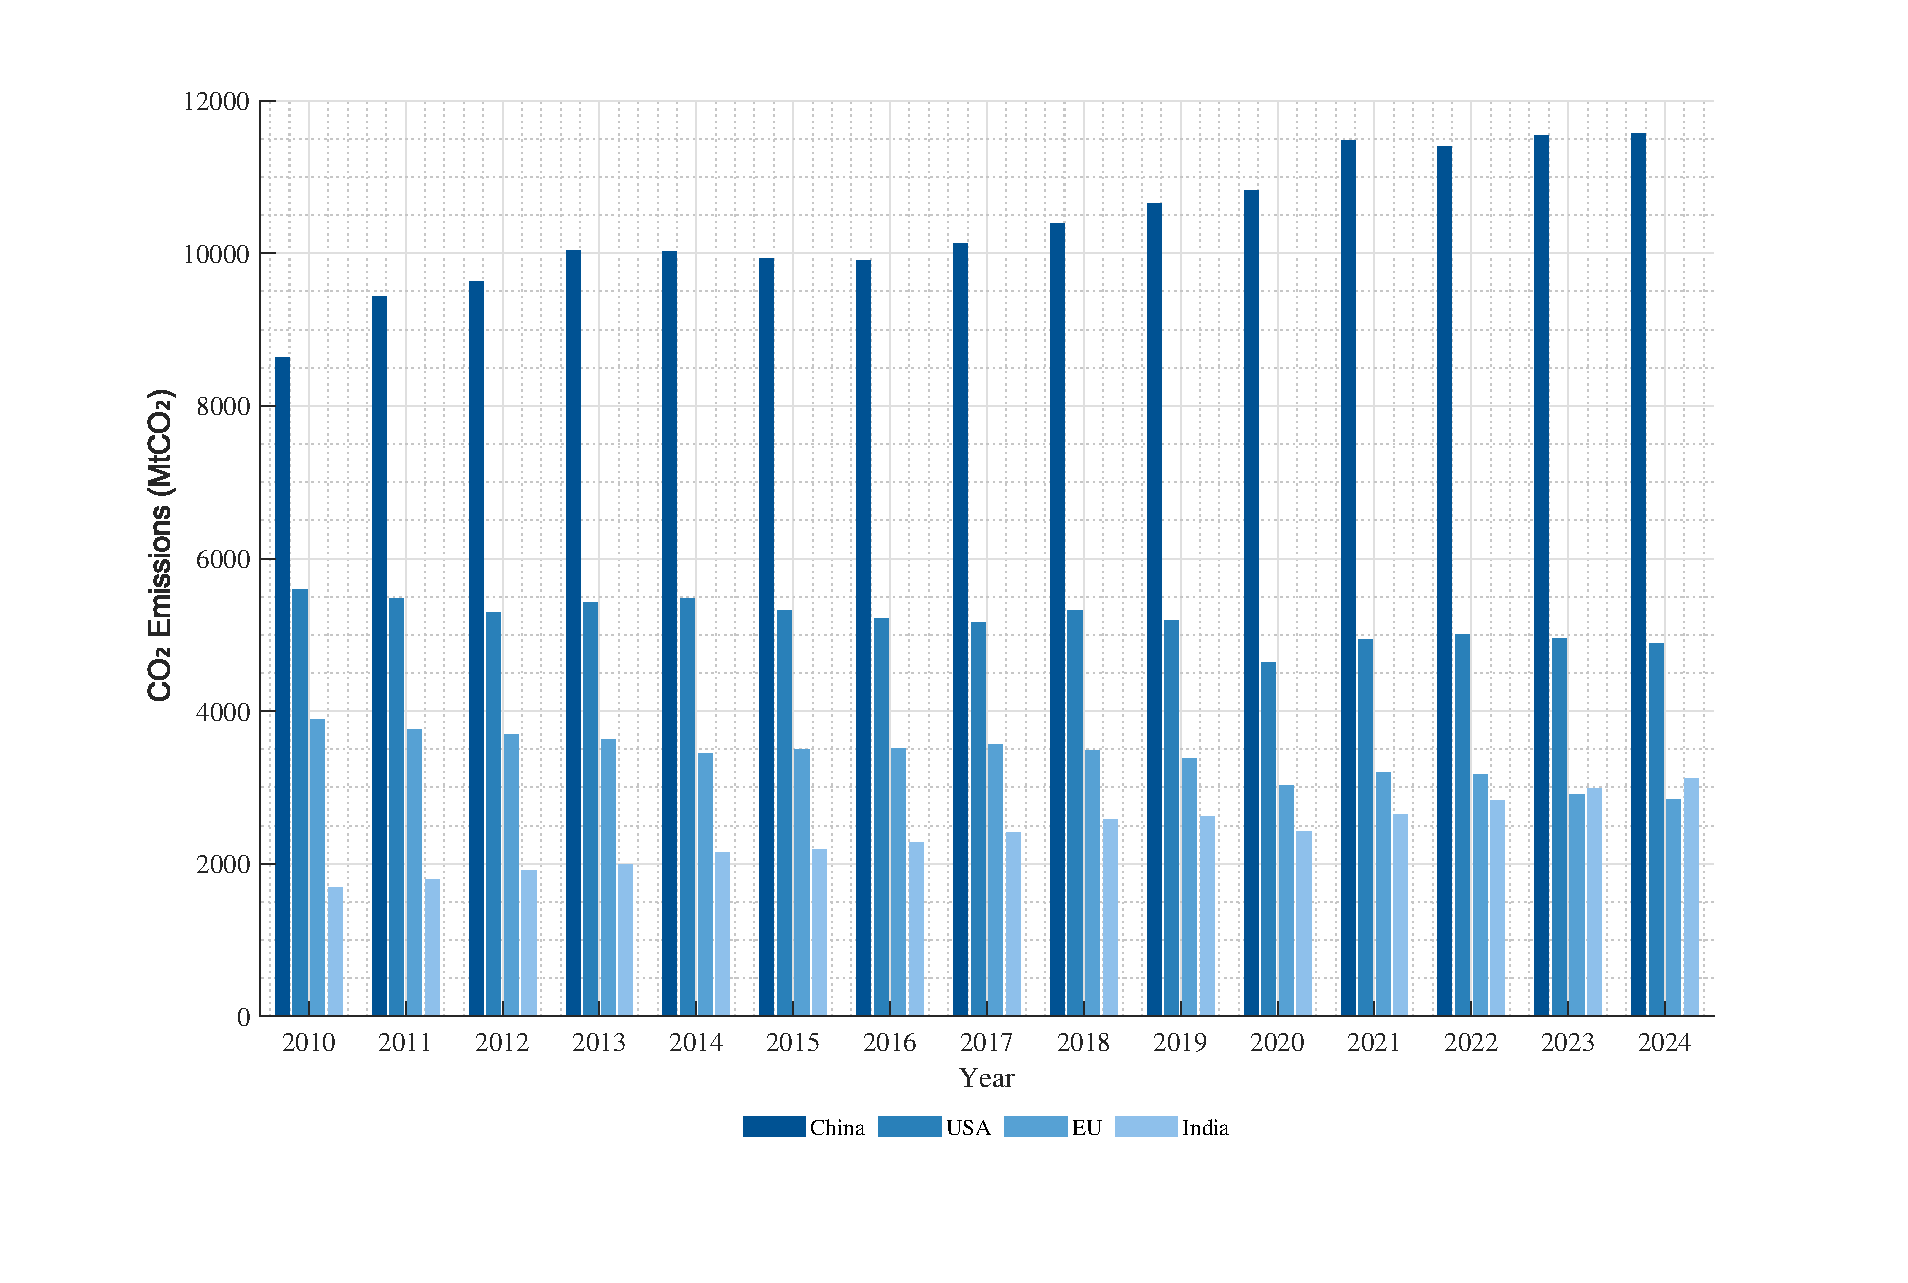
\includegraphics[width=0.9\linewidth]{global_co2_emissions.eps}
    \label{fig:co2_emissions}
\end{figure}


There are three primary pathways for decarbonizing aviation:

The first pathway involves continuing to use fossil-based kerosene while improving combustion efficiency for emission reduction, coupled with direct air capture and carbon sequestration elsewhere. Although sequestration costs are significantly lower than those for renewable kerosene, the carbon reduction potential of conventional technological improvements like fuel efficiency is limited, and this may not represent a fully sustainable long--term solution.

The second pathway adopts hydrogen and renewable electricity as aircraft energy sources. However, the application of electrification and hydrogen energy requires substantial modifications to aircraft structures, making large--scale adoption difficult in the short to medium term.

The third pathway is the use of Sustainable Aviation Fuel (SAF). SAF shares similar physical characteristics with conventional aviation kerosene yet can reduce CO2 and CH4 emissions by 50\%--90\%, without requiring major alterations to aircraft systems or fuel supply infrastructure. According to projections by the International Air Transport Association (IATA), the aviation industry will achieve net--zero emissions by 2050, and the adoption of SAF is widely regarded as the most feasible technological pathway for aviation decarbonization in the coming decades.

The international community has already taken action. Major economies such as the European Union, the United Kingdom, and the United States are adopting a 'legislation--first' approach, establishing policy frameworks including mandatory blending mandates, certificate trading, and tax credits. These measures aim to create stable market demand, attract private investment, and accelerate the maturation and expansion of the SAF industrial chain.

In contrast, although China has incorporated SAF development into its 14th Five--Year Plan for Civil Aviation Green Development \cite{caac2021} and has successfully completed multiple rounds of demonstration applications and pilot projects, its industrial scale remains far below the level required to achieve its Nationally Determined Contributions. China's SAF technology is still in its preliminary research stage.

The core contradiction lies in the fact that recent technological verification and pilot projects have failed to catalyze a self-sustaining commercial market.

This policy brief aims to diagnose the root causes of this contradiction and propose solutions. We focus on answering two questions: First, why has China's SAF industry encountered a 'scale--up bottleneck' even after completing technological demonstrations? Second, how can precise policy design quickly bridge the critical path from demonstration to commercialization?
The analysis in this brief will focus on policies and market mechanisms, primarily targeting policymakers and key market participants who need to allocate public resources and formulate industry rules accordingly. The brief will sequentially analyze three key bottlenecks: Firstly, the lack of legally binding market demand signals; Secondly, a fragile and regionally mismatched feedstock supply chain; Thirdly, missing cost incentive mechanisms and a disconnect between the accounting system and market tools. For each bottleneck, this policy brief will assess feasible international policy options and propose implementation pathways and recommendations tailored to China's national conditions and regulatory framework. The economic implications of scaling SAF are significant, as discussed in Timmons and Terwel \cite{timmons2022} and Sandford and Malins \cite{sandford2024} for the UK context. The technical and policy progress globally is further detailed by IEA Bioenergy \cite{iea2024} and IRENA \cite{irena2024}.

%%%%%%%%%%%%%%%%%%%%%%%%%%%%%%Overview of the problem Box%%%%%%%%%%%%%%%%%%%%%%%%%%%%%%
\section{Overview of the problem}
\subsection{Targets exist, but without binding mandate}
The 'Special Plan for Civil Aviation Green Development during the 14th Five-Year Plan Period' \cite{caac2021} has set the industry target of 'cumulative consumption of sustainable aviation fuel (SAF) reaching 50,000 tons by 2025', but it has not established a mandatory blending ratio nationwide or a unified carbon intensity threshold. This is a directional goal rather than a legal constraint, making it difficult to form a predictable rigid demand. During the same period, more focused application pilots and demonstrations have been promoted. The competent authorities have released the phased arrangements for the pilot projects, indicating that the overall situation is still in the 'exploration --- verification' stage. On the industrial side, \textit{China's Sustainable Aviation Fuel --- The Road to Carbon Neutrality for the Aviation Industry} (Deloitte, 2023) \cite{deloitte2023} has summarized that as of May 2023, the total operating and planned production capacity in China is approximately 160--180 million tons per year, mainly based on the HEFA route, confirming the characteristic of 'having projects and early implementation'. Without strong constraints, the production capacity is difficult to steadily increase, and the renovation of airport storage and independent tank storage is also difficult to justify the investment return.

\subsection{Raw material supply constraints and cross-border mismatches}
At present, the most mature and accessible raw material is still waste edible oil (UCO), but it faces practical constraints such as scattered sources, small recycling radius, high collection and transportation costs, and limited recoverable volume. Moreover, driven by international market prices and demand, UCO has the risk of outflow, which raises domestic raw material prices and weakens supply stability. Specifically, in 2024 China collected and processed approximately 5.4 million tonnes of used cooking oil (UCO), with 55\% (2.95 million tonnes) exported and 45\% (2.45 million tonnes) consumed domestically. The exports primarily flowed to the United States (43\%) and the European Union (35\%) \textbf{(Table 1)}. This trade structure indicates that domestically available feedstock continues to be absorbed by external demand, driving up raw material costs and supply uncertainties for local SAF projects.


{\arrayrulecolor{schoolblue}%
\begin{table}[htbp]
\centering
\caption{ {\color{schoolblue}China UCO (Used Cooking Oil) 2024 Overview — Integrated Table}}
\label{tab:ucosummary}

% 使用 booktabs 的 \toprule, \midrule, \bottomrule 来代替 \hline
% 使用 \rowcolor{...} 为第一行设置浅色背景
\begin{tabular}{lrr}
\toprule
\rowcolor{schoolbluelight} % 浅蓝色背景
\textbf{A. 2024 total \& allocation (Unit: Mt; shares vs total)} & & \\
\midrule
\textbf{Item} & \textbf{Volume (Mt)} & \textbf{Share} \\
\cmidrule(lr){1-3}
Total collected \& processed & 540.0 & 100\% \\
Domestic use & 245.0 & 45\% \\
Exports & 295.0 & 55\% \\
\midrule
\rowcolor{schoolbluelight} % 浅蓝色背景
\textbf{B. 2024 export destinations (Base: exports 295.0 Mt)} & & \\
\midrule
\textbf{Export destination (Base: Exports 295.0 Mt)} & \textbf{Volume (Mt)} & \textbf{Share} \\
\cmidrule(lr){1-3}
United States & 126.8 & 43\% \\
European Union (e.g., NL, ES) & 103.2 & 35\% \\
Singapore & 35.4 & 12\% \\
Others & 29.5 & 10\% \\
\textbf{Total} & \textbf{295.0} & \textbf{100\%} \\
\midrule
\rowcolor{schoolbluelight} % 浅蓝色背景
\textbf{C. Exports by year (Base: cumulative 655.6 Mt; 2024 = 45\%)} & & \\
\midrule
\textbf{Exports by year (Base: cumulative 655.6 Mt)} & \textbf{Volume (Mt)} & \textbf{Share} \\
\cmidrule(lr){1-3}
2024 & 295.0 & 45\% \\
2023 (derived) & 209.8 & 32\% \\
2022 \& earlier (derived) & 150.8 & 23\% \\
\textbf{Cumulative (2022 \& earlier - 2024)} & \textbf{655.6} & \textbf{100\%} \\
\bottomrule
\end{tabular}

\medskip
\footnotesize Note: Unit = million tonnes (Mt). Source: China's General Administration of Customs.
\end{table}}

From a historical composition perspective, the 2024 export volume already accounts for 45\% of cumulative exports, indicating significantly strengthened external demand in recent years. Without urgent efforts to expand the available feedstock pool through cross--border collaboration and attribute accounting, while improving domestic collection and traceability systems, production ramp--up will remain constrained and airlines will struggle to consistently execute their blending schedules.


The research report \textit{Research on the Development of Sustainable Aviation Fuel Industry in China} points out: In the medium and long term, while consolidating the foundation of UCO, it is necessary to gradually expand to various raw materials such as agricultural and forestry waste, and improve the cross-regional collection and transportation as well as quality traceability system. Otherwise, the 'raw material bottleneck' will directly restrict the ramp-up of production capacity and continuous supply. Deloitte's report \textit{China's Sustainable Aviation Fuel - The Road to Carbon Neutrality for the Aviation Industry} \cite{deloitte2023} based on customs and other data shows the synchronous growth of UCO exports and domestic uses, and gives theoretical upper limit estimates of potential available raw materials and corresponding SAF production capacity (about 46 million tons per grade upper limit), while emphasizing that the potential needs to be transformed into available supply depends on the collection network, traceability and priority rules. This directly affects the annual blending plans of airlines and long-term supply contracts of suppliers. Without a stable, traceable and large-scale raw material system, it is difficult to support stable blending and long-term supply contracts, and the costs and risks of the upstream and downstream of the industry cannot be accepted by banks and investors.

\subsection{High costs, weak incentives, accounting---pricing misalignment}
China's Study on Sustainable Aviation Fuel Industry Development \cite{tian2025} indicates that the unit cost of multiple SAF production pathways is approximately 2--6 times that of conventional petroleum-based jet fuel, making the 'green premium' a core barrier to commercialization. Concurrently, insufficient fiscal/tax incentives and the absence of price transmission mechanisms make it difficult for airlines and fuel producers to absorb this cost differential. Deloitte's report, \textit{Sustainable Aviation Fuel in China -- Aviation's Path to Carbon Neutrality} \cite{deloitte2023}, further cites the price point and abatement cost for neat SAF (approximately \$8.67 per gallon; \textasciitilde\$1,000--1,200 per ton of CO\textsubscript{2}), analyzing key cost drivers such as feedstock availability, economies of scale, policy incentives, value chain efficiency, and reporting standards. The report underscores that reliance on demonstration projects alone is insufficient for spontaneous industry growth.

On the regulatory and accounting front, China has released the 'Aviation Fuel---Methods and Requirements for Product Carbon Footprint Quantification---Part 1: General Rules' (MH/T 6138.1---2025) \cite{caac2025}, which standardizes lifecycle accounting rules and reporting frameworks. However, these rules are not yet systematically linked to price and market mechanisms such as subsidies, credits, or settlement. Consequently, when companies enter into medium- to long-term supply agreements or engage in green finance and performance-based settlements, they lack a coherent loop integrating accounting, incentives, and settlement.

In the absence of a verifiable, bankable, and capable of supporting final settlement closed-loop system, the price gap cannot be reliably covered. This undermines investment and financing confidence, hindering the scale-up of the industry.

%%%%%%%%%%%%%%%%%%%%%%%%%%%%%%Examination of the findings and options%%%%%%%%%%%%%%%%%%%%%%%%%%%%%%

\section{Examination of the findings and options}

\subsection{Establish a statutory SAF blending mandate}
Following the UK's Sustainable Aviation Fuel (SAF) mandate, obligations will be set based on a total proportion starting from 2025. The obligations will be 2\% in 2025, 10\% in 2030, and 22\% in 2040. Certificates that can be traded will be used as the compliance medium, and a buy-out price (buy-out price) will be set as the upper limit for compliance costs (obligation £4.70/L, PtL sub-obligation £5.00/L). Any shortfall can be purchased at the upper limit to prevent cost runaway due to extreme shortages. The regulatory framework is parallel to the RTFO, and technical and compliance guidelines are provided to clearly define qualified fuels, verification, and compliance processes, as well as the implementation path in China. The economic feasibility of such mandates is explored in detail by Sandford and Malins \cite{sandford2024}.

\subsubsection{China's landing method}
In terms of law-making and time planning, the Civil Aviation Administration, the National Development and Reform Commission, and the Ministry of Finance jointly proposed the 'Management Measures for Obligatory Sustainable Aviation Fuels', clearly stating that in 2026, several hub airports will be piloted, in 2027, the obligation will be implemented nationwide, initially covering international departure routes, and by 2030, it will be expanded to trunk domestic routes. In terms of the market mechanism, a national registration and settlement platform for SAF qualified certificates (S-Certs) will be established; the certificates can be traded, with the selling price set as the upper limit of the cost, and adjusted according to the assessment year. In terms of verification and supervision, a unified definition of qualified fuels and sustainable standards will be established, the entire process of certificate issuance and cancellation will be subject to MRV, and equivalent recognition rules will be set for cross-border supply, and it will be compatible with CORSIA and domestic standards.

\subsubsection{Expected effect}
Form a rigid and predictable demand curve, facilitating airlines to sign long-term supply and purchase contracts, and forcing the upgrading of production capacity and storage and transportation facilities at airports; the purchase price sets an upper limit for compliance costs, reducing the premium for policy uncertainty.

\subsection{Boosting SAF Scale-Up through Feedstock Cooperation and National Accounting}





































According to the regional collaboration approach in \textit{Sustainable Aviation Fuels in Southeast Asia} (IRENA (2024)) \cite{irena2024}: On one hand, sign a cross-border raw material and attribute collaboration framework with the major raw material source countries of UCO and agricultural and forestry residues in Southeast Asia, and unify the sustainability and traceability rules; on the other hand, establish a national 'book-and-claim' platform to separate attributes from physical flows, enabling raw materials to be processed locally within the region, but the emission reduction attributes can be issued, traded, and offset through the platform, allowing Chinese airlines to use them in compliance. Form a rigid and predictable demand curve, facilitating airlines to sign long-term supply and purchase contracts, forcing capacity expansion and storage and transportation renovations on the part of airports; the purchase price sets an upper limit for compliance costs, reducing the premium for policy uncertainty.

\subsubsection{China's landing method}
On Regulation and Platform: The Civil Aviation Administration, State Administration for Market Regulation, and General Administration of Customs shall jointly issue guidelines for Attribute Certificates (A-Certs), designate a national-level clearing platform, and implement unified numbering, one-time issuance, one-time cancellation, and full-chain auditing.

On Cross-Border Coordination: China will sign Memoranda of Understanding with Indonesia, Malaysia, Thailand, and other nations to mutually recognize feedstock and emission attributes. It will align with ISCC CORSIA/domestic standards to establish a closed-loop process covering overseas procurement, border entry, and certificate issuance.

Furthermore, these efforts will be integrated into domestic policy: book-and-claim outcomes will be incorporated into the eligibility criteria for airline compliance and fiscal or tax incentives, translating emission reduction initiatives into actionable and accountable measures.

\subsubsection{Expected effect}
Alleviate the outflow and shortage of UCO within the country, expand the regional resource pool; replace the costly full physical return with low-friction attribute settlement, accelerate blending and cost reduction.

\subsection{Implement CI-based producer support}
Drawing on the policy in the 'Internal Revenue Code \& 45Z Clean Fuel Production Credit' of the United States \cite{irs2025}, where subsidies are given based on the lifecycle carbon intensity (CI) for clean transportation fuels produced and sold domestically. In China, the 'CI tiered subsidy' approach can be adopted. The lower the CI value of an enterprise, the higher the subsidy. And all the settlement and auditing parts should be aligned with our country's industry standards.

\subsubsection{China's landing method}
In terms of subsidy design, the fiscal and tax departments have issued a policy for production subsidies based on CI classification, which only pays to SAF that is produced domestically and undergoes verification. And it sets an annual total amount and a single-factory upper limit. In terms of accounting and auditing: The unified LCA framework is based on the 'Quantification Method and Requirements for Carbon Footprint of Aviation Fuel Products --- Part 1: General Provisions' (MH/T 6138.1---2025) \cite{caac2025}, and third-party verification is introduced. In terms of linkage tools, the CI results are embedded in certificate pricing and green financial products, and are used as the benchmark for credit allocation or emission reduction accounting.

\subsubsection{Expected effect}
The implementation of these policies will bridge the cost gap, improve the viability of marginal projects, and create a dual-driven dynamic of 'demand and supply' in conjunction with mandated blending. The design of the Carbon Intensity (CI) bracket policy further incentivizes enterprises to adopt lower-carbon feedstocks and production processes.


%%%%%%%%%%%%%%%%%%%%%%%%%%%%%%Policy Recommendations%%%%%%%%%%%%%%%%%%%%%%%%%%%%%%

\section{Policy Recommendations}
This part would be written and presented in final term. Thanks!

%%%%%%%%%%%%%%%%%%%%%%%%%%%%%%Reference%%%%%%%%%%%%%%%%%%%%%%%%%%%%%%
\newpage
\begin{thebibliography}{9}

% 1. caac2025 (First cited in Executive Summary)
\bibitem{caac2025}
Civil Aviation Administration of China (CAAC). (2025, August 9). \textit{Greenhouse gases---Quantification requirement and method of product carbon footprint---Aviation fuel---Part 1: General rules} [MH/T 6138.1 2025]. Civil Aviation Administration of China.
\url{https://www.caac.gov.cn/XXGK/XXGK/BZGF/HYBZ/202508/t20250812_228248.html    }

% 2. caac2021 (Second cited in Introduction)
\bibitem{caac2021}
Civil Aviation Administration of China. (2021, December 21). \textit{Notice on the issuance of the ``14th Five-Year Plan'' for the green development of civil aviation} [Civil Aviation Administration of China Document No. 54]. Civil Aviation Administration of China.
\url{https://www.caac.gov.cn/XXGK/XXGK/FZGH/202201/t20220127_211345.html    }

% 3. timmons2022 (Third cited in Introduction)
\bibitem{timmons2022}
Timmons, D., \& Terwel, R. (2022). Economics of aviation fuel decarbonization: A preliminary assessment. \textit{Journal of Cleaner Production}, 369, Article 133097.
\url{https://doi.org/10.1016/j.jclepro.2022.133097    }

% 4. sandford2024 (Fourth cited in Introduction)
\bibitem{sandford2024}
Sandford, C., \& Malins, C. (2024, August 28). \textit{Vertical take-off? Cost implications and industrial development scenarios for the UK SAF mandate}. International Council on Clean Transportation.
\url{https://theicct.org/publication/cost-implications-industrial-development-scenarios-uk-saf-mandate-aug24/    }

% 5. iea2024 (Fifth cited in Introduction)
\bibitem{iea2024}
IEA Bioenergy. (2024). \textit{Progress in Commercialization of Biojet/Sustainable Aviation Fuels (SAF): Technologies and policies}.
\url{https://www.ieabioenergy.com/blog/publications/progress-in-commercialization-of-biojet-sustainable-aviation-fuels-saf-technologies-and-policies/    }

% 6. irena2024 (Sixth cited in Introduction, then again in Examination section)
\bibitem{irena2024}
International Renewable Energy Agency (IRENA). (2024). \textit{Sustainable aviation fuels in Southeast Asia: A regional perspective on bio-based solutions}. International Renewable Energy Agency.

% 7. deloitte2023 (Seventh cited in Overview section, then again)
\bibitem{deloitte2023}
Deloitte. (2023). \textit{Sustainable aviation fuels (SAF) in China: Checking for take-off}. Deloitte.
\url{https://www.deloitte.com/cn/zh/Industries/energy/perspectives/saf-in-china.html    }

% 8. tian2025 (Eighth cited in Overview section)
\bibitem{tian2025}
Tian, L., Liu, X., Lyu, J., Yang, X., You, C., \& Chen, X. (2025). Development strategy of sustainable aviation fuel. \textit{Strategic Study of CAE}, 27(2), 49--61.
\url{https://doi.org/10.15302/J-SSCAE-2024.07.022    }

% 9. irs2025 (Ninth cited in Examination section)
\bibitem{irs2025}
Internal Revenue Service. (2025, January 8). \textit{Notice 2025-10: Clean fuel production credit; request for public comments}. Internal Revenue Service.
\url{https://www.irs.gov/pub/irs-drop/n-25-10.pdf    }

\end{thebibliography}

\end{document}